\chapter*{Chapitre 1 : Présentation de l'Organisme d'Accueil}
\addcontentsline{toc}{chapter}{Chapitre 1 : Présentation de l'Organisme d'Accueil}
\thispagestyle{fancy}
\setcounter{section}{0}
\newpage

\section{Introduction}

Dans le cadre de mon stage de fin d'études au sein de l'International Academy of Artificial Intelligence (IAAI Academy) à Casablanca, ce chapitre présente en détail l'organisme d'accueil. Il définit le contexte institutionnel, pédagogique et technologique dans lequel mon immersion professionnelle s'est déroulée, offrant une vue d'ensemble indispensable pour appréhender les missions et compétences mobilisées.

Ce chapitre permettra de :
\begin{itemize}
  \item Identifier l'origine et la mission de l'IAAI Academy
  \item Décrire sa structure organisationnelle et ses ressources matérielles et humaines
  \item Mettre en lumière son positionnement innovant à l'intersection de l'intelligence artificielle, du développement Web et mobile, et de l'éducation
\end{itemize}

\section{Historique et Genèse de l'IAAI Academy}

\begin{itemize}
  \item \textbf{Date de création :} Fondée en 2024 à Casablanca par un collectif de docteurs et d'experts en intelligence artificielle, animés par la volonté de transformer le paysage éducatif marocain.
  
  \item \textbf{Contexte et motivations :} Face à l'évolution rapide du secteur de l'IA et aux défis du XXIᵉ siècle, l'IAAI Academy se donne pour objectif de :
  \begin{itemize}
    \item Renforcer les compétences nationales en IA
    \item Réinventer la pédagogie grâce à des solutions assistées par IA
    \item Devenir un pôle de recherche appliquée et d'innovation au service des étudiants, des enseignants et des entreprises
  \end{itemize}
\end{itemize}

\section{Mission, Vision et Valeurs}

\begin{figure}[H]
  \centering
  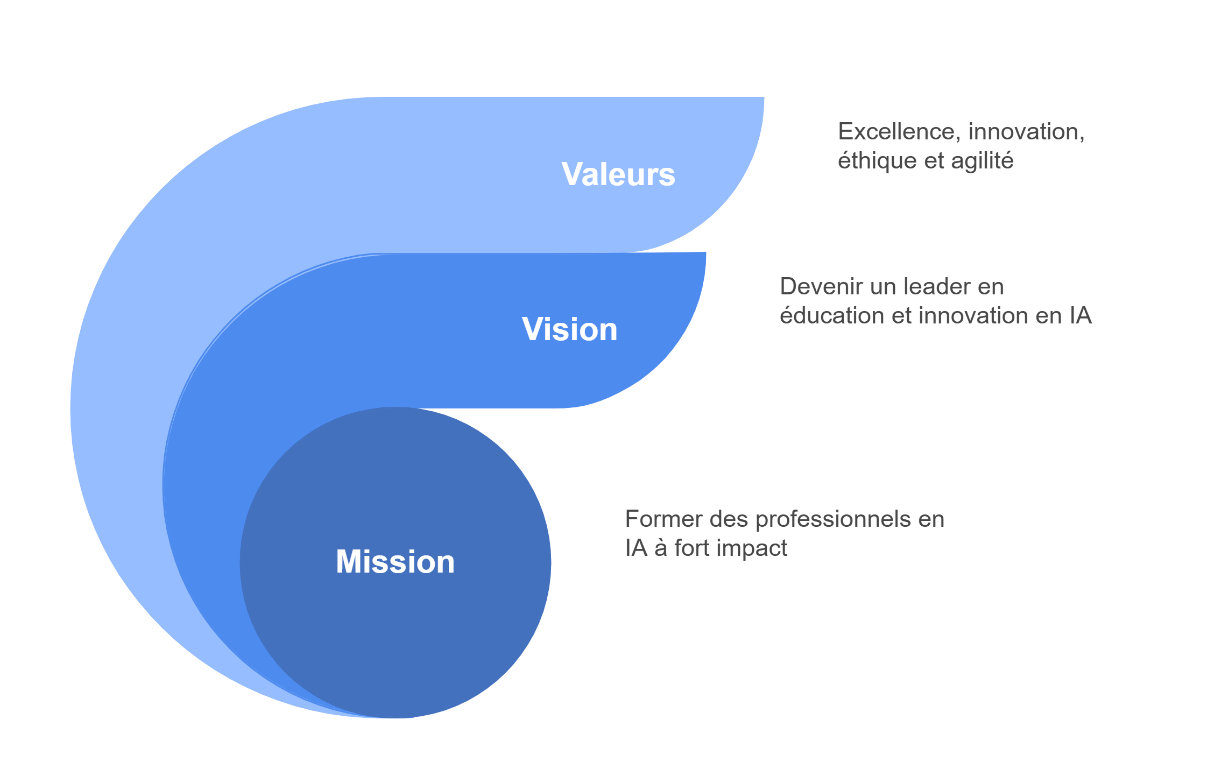
\includegraphics[width=0.8\textwidth]{images/mession.png}
  \caption{\textbf{Mission et vision de l'IAAI Academy}}
  \label{fig:mission}
\end{figure}

\begin{itemize}
  \item \textbf{Mission :} Former des professionnels capables de concevoir, déployer et piloter des solutions d'intelligence artificielle à fort impact, en s'appuyant sur une pédagogie innovante et des outils technologiques avancés.
  
  \item \textbf{Vision :} Devenir la référence au Maroc et en Afrique pour l'enseignement supérieur, l'innovation pédagogique et la recherche appliquée en IA, tout en contribuant à la transformation digitale du secteur éducatif.
  
  \item \textbf{Valeurs :}
  \begin{itemize}
    \item Excellence académique et exigence professionnelle
    \item Innovation pédagogique via l'intégration des technologies IA
    \item Éthique et esprit collaboratif
    \item Agilité et adaptabilité aux évolutions technologiques
  \end{itemize}
\end{itemize}

\section{Structure Organisationnelle et Gouvernance}

\begin{figure}[H]
  \centering
  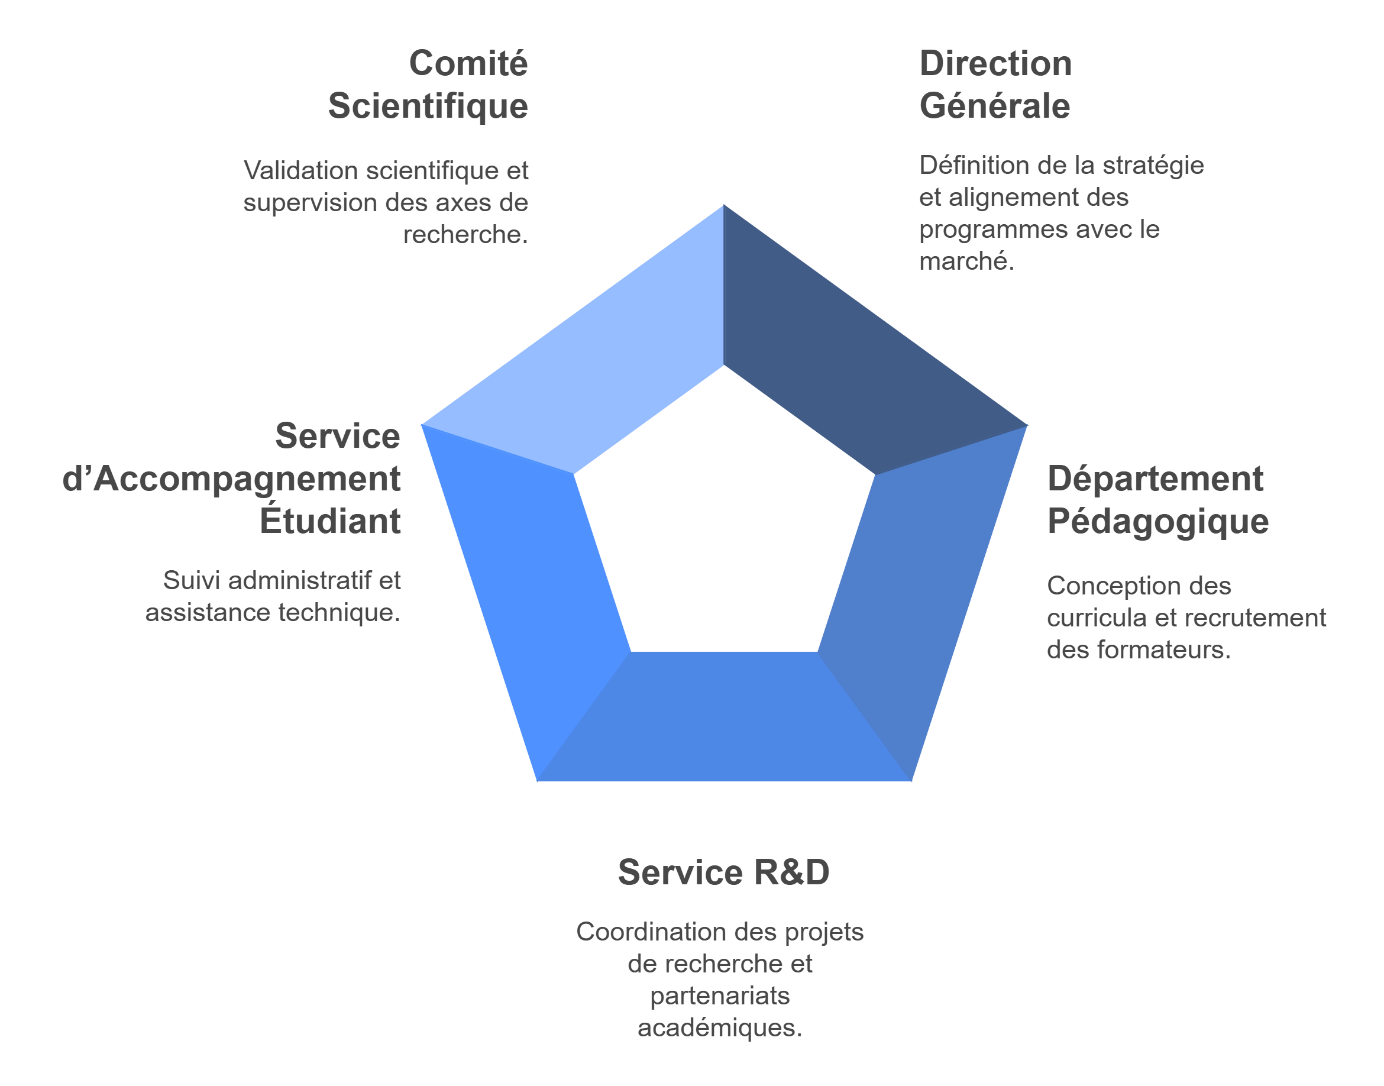
\includegraphics[width=0.9\textwidth]{images/Structure Organisationnelle et Gouvernance.png}
  \caption{\textbf{Organigramme et structure de gouvernance de l'IAAI Academy}}
  \label{fig:structure}
\end{figure}

L'IAAI Academy dispose d'une structure organisationnelle efficace, composée de plusieurs départements et unités qui travaillent en synergie pour atteindre les objectifs de l'institution. La gouvernance est assurée par un conseil d'administration et un comité exécutif qui définissent les orientations stratégiques et supervisent la mise en œuvre des projets.

\section{Offres de Formation et Domaines d'Intervention}

\begin{figure}[H]
  \centering
  \includegraphics[width=0.9\textwidth]{images/Offres de Formation et Domaines d'Intervention.png}
  \caption{\textbf{Panorama des formations et domaines d'expertise de l'IAAI Academy}}
  \label{fig:formations}
\end{figure}

\begin{itemize}
  \item \textbf{Formations professionnelles en IA et Data Science :}
  \begin{itemize}
    \item Modules intensifs (Python, Machine Learning, Deep Learning, NLP, vision par ordinateur)
    \item Certifications reconnues (IBM, Microsoft, Google, Coursera)
  \end{itemize}
  
  \item \textbf{Préparation aux concours post-bac :}
  \begin{itemize}
    \item Parcours pour médecine, pharmacie, ENSA/ENSAM, ENCG
    \item Formats présentiel, à distance ou hybride, avec examens blancs et coaching
  \end{itemize}
  
  \item \textbf{Soutien scolaire individualisé :}
  \begin{itemize}
    \item Cours sur mesure en mathématiques, physique-chimie, SVT et informatique
    \item Suivi des progrès, méthodes de travail et préparation aux examens
  \end{itemize}
  
  \item \textbf{Consulting et prestations IA :}
  \begin{itemize}
    \item Développement de chatbots, automatisation de processus et analyses prédictives
    \item Accompagnement à la transformation numérique
  \end{itemize}
  
  \item \textbf{Clubs technologiques et ateliers jeunesse :}
  \begin{itemize}
    \item Initiation à la programmation, robotique éducative et réalité augmentée
    \item Projets ludiques pour stimuler l'innovation dès le plus jeune âge
  \end{itemize}
\end{itemize}

\section{Pédagogie et Méthodes d'Apprentissage}

\begin{figure}[H]
  \centering
  \includegraphics[width=0.9\textwidth]{images/Pédagogie et Méthodes d'Apprentissage.png}
  \caption{\textbf{Approche pédagogique innovante de l'IAAI Academy}}
  \label{fig:pedagogie}
\end{figure}

L'IAAI Academy adopte une approche pédagogique innovante, intégrant les technologies d'intelligence artificielle pour personnaliser l'apprentissage et optimiser l'acquisition des compétences. Cette méthode combine enseignement théorique, pratique intensive et projets concrets, enrichis par des outils d'évaluation continue et d'adaptation du contenu au profil de chaque apprenant.

\section{Impact de mon Stage}

Ce stage m'a permis de :
\begin{itemize}
  \item M'immerger dans un environnement professionnel concret, en participant à des projets IA et pédagogiques
  \item Renforcer mes compétences en data science et technologies IA, ainsi qu'en développement Web (React) et mobile (React Native)
  \item Collaborer au sein d'une équipe pluridisciplinaire, développant ma capacité d'adaptation et de communication
  \item Adopter une posture critique et réflexive, afin de proposer des solutions innovantes et répondre aux enjeux réels du terrain
\end{itemize}

\section{Conclusion}

L'IAAI Academy a offert un cadre d'apprentissage et de recherche exemplaire, conjuguant ressources innovantes, démarche pédagogique assistée par IA et infrastructures technologiques avancées. Ce stage m'a non seulement permis de consolider mes compétences et de comprendre les enjeux de l'intégration de l'IA en contexte réel, mais il m'a également ouvert de nouvelles perspectives professionnelles et académiques dans le domaine de l'intelligence artificielle appliquée à l'éducation. 